%!TEX root = ../../thesis.tex

\section{Detecting atmospheres}
To help characterize an exoplanet, a detection of its atmosphere can provide useful information. After the detection of exoplanets and the measurement of bulk properties, detecting their atmospheres is the next step. The detection of planetary atmosphere is difficult due to the low planet-to-star flux ratio. This requires high precision instrumentation to detect. For example the planet-to-star flux ratio in the optical is $\approx 10^{-4}$ for a hot Jupiter with a 3 day orbit, in which the main component is reflected star light. In the infrared the thermal emission of the planets dominate and the flux ratio rises to $\approx 10^{-3}$. These flux ratios requires observations with signal-to-noise ratios of $10^4$ and $10^3$ in the optical and infrared respectively to achieve a planetary signal at the same level as the noise level. Only just at the capabilities of the current generation of technology, and with very long observation cost.


Several photometric and high-resolution spectroscopic techniques are showing promising results; detailed in the following sections.


\subsection{Occultation and phase variations}
Exoplanet atmospheres are analysis by considering the observed light as containing two components, not only light from the star but also light from the planet, albeit at a much lower flux level.
To help visualize and discuss the components of exoplanet atmospheres \fref{fig:transits_and_occultations} is provided showing a transiting planet in orbit around a star, in which the planet also passes behind the star causing an occultation. The planet is shown at several positions of the orbit indicating the proportion of dayside and night side observed.  Below the star and planet is a diagram showing the changing flux variation over time, following the orbit. 

\begin{figure}
    \centering
    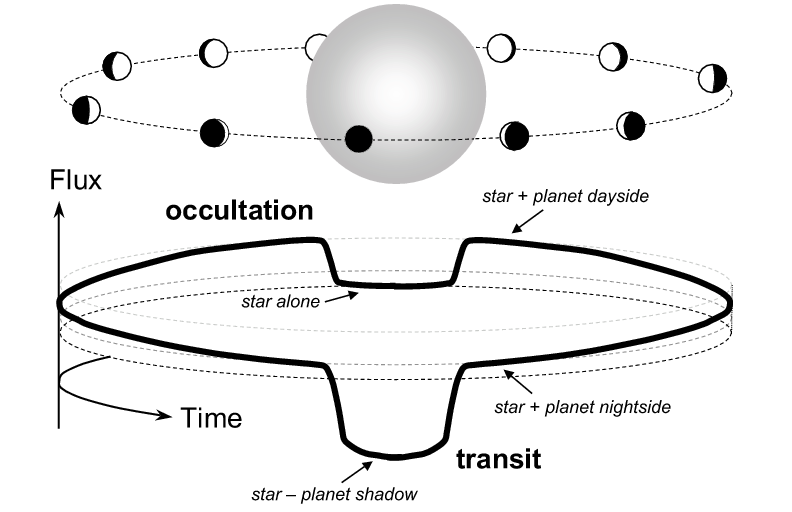
\includegraphics[width=0.6\linewidth]{./figures/introduction/circular_diagram.png}
    \caption{Illustration of the flux contribution from a star and planet in a transiting exoplanet system throughout its orbit. Credit~\citet{winn_transits_2010}}
    \label{fig:transits_and_occultations}
\end{figure}

Throughout the orbit of the planet there is a variation in the planetary flux due to the alternating day/night side of the planet observed.
There are multiple components of the planetary flux, reflection and emission,  that can be analysed with multi-band phase curves \citep[e.g.][]{knutson_characterizing_2009, esteves_optical_2013}. Optical phase curves will mostly show the reflected light from the day side of the planet, allowing modelling the atmospheric albedo (fraction of light reflected by the atmosphere), and can provide details on the atmospheric scattering~\citep{madhusudhan_analytic_2012} and aerosol composition~\citep{oreshenko_optical_2016} through the optical phase function (day/night fraction). Thermal emission of the planet will provide stronger modulation of infrared phase curves and can provide insights into the atmospheres thermal
structure and heat circulation~\citep{ goodman_thermodynamics_2009, koll_temperature_2016 }.


An example of phase variations in infrared spectra obtained with the Hubble Space telescope 
\begin{figure}
    \centering
    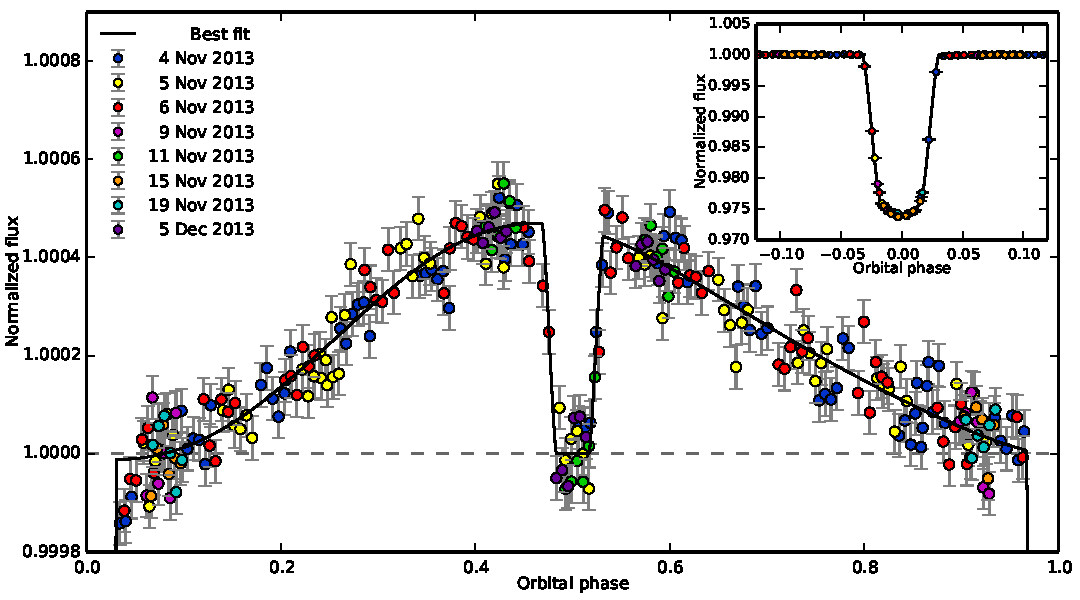
\includegraphics[width=0.6\linewidth]{figures/introduction/stevenson_phasecurve2014}
    \caption{Band integrated phase variation of WASP-43b from the HST - \cite{stevenson_thermal_2014}. The primary transit is inset top right.
        The peak of brightness occurs before the secondary transit, indicating heat distribution of the }
    \label{fig:stevensonphasecurve2014}
\end{figure}



The photometric and spectroscopic technique can be understood 
photometric and high-resolution spectroscopicphotometric and high-resolution spectroscopic

Secondary transit and phase variations are an extension of the transit method, requiring higher precision to detect the reflection and thermal emission of the exoplanet. The star with orbiting exoplanet is photometrically monitored over the whole orbit. An example diagram of phase variation is shown in \fref{fig:transits_and_occultations} as the solid black line. Starting with the primary transit at the bottom, in which the planet is blocking the star. The light measured during transit is not only the unblocked light from the star but also the thermal emission from the night side of the planet. Immediately before and after transit there will be the full flux from the star plus the emission from the night side of the planet. As the planet orbits around the star the fraction of the day side of the planet visible will change up to maximum when the full day side of the planet is visible. If the alignment is correct the planet will pass behind the star causing an occultation. At this point the only light received is from the star alone.

The depth of the occultation is a measure of the flux from the day side of the planet which can indicate the atmospheric reflection and thermal emission of the planets atmosphere.
Continuing on in the orbit the phase of combined star + planet again reduces as more of the night side faces Earth.

\fref{fig:stevensonphasecurve2014} shows a real example of the phase folded light curve measured with the HST over several orbits~\citep{stevenson_thermal_2014}.

The primary transit is shown inset with a depth of 2.5\%. The phase variation out of primary transit reaches a maximum of around 0.04\%. The occultation occurs at a phase of 0.5 but it is clearly noticeable that the peak of brightness in the light phase curve slightly leads the occultation. This indicates that the brightest point on the planet is not directly towards the planet. and there is heat redistribution.

thermal profile/phase of hot spot.



\subsection{Transmission spectroscopy}
radius changes with wavelength, extra absorption during transit can give molecular composition.

snellen  et al


Transit and occulations~\citet{winn_transits_2010}

Detection of winds



\citep{hoeijmakers_atomic_2018} detected Iron and titanium in ultra-hot Jupiter with Teff 4000K during transit.high resolution specrosopy






\subsection{High resolution spectroscopy}
Snellen  Brogi, de Kok

Cross correlation mle  \citet{piskorz_evidence_2016}


For non-transiting planets ...

